Think about what ideal $3\times3$ patch from each of the input channels would maximally activate the corresponding $3\times3$ filter. Fill in these maximally activating patches in the area below. If there are any unused cells (i.e., cells that would not make any difference) after completing the process in the provided tables, place an $\times$ in them. (2pts)

\begin{figure}[H]
	\centering
	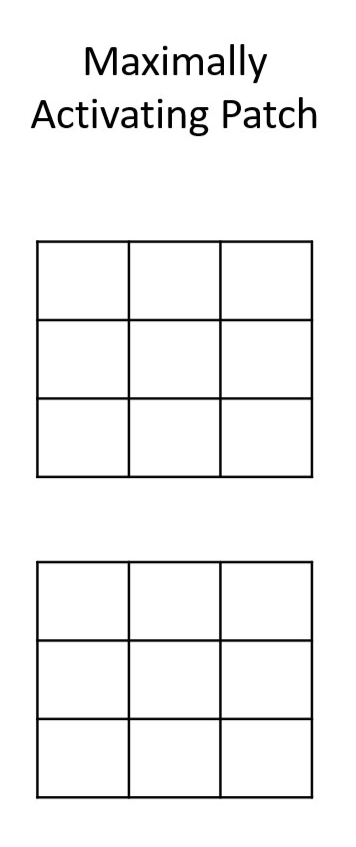
\includegraphics[width=.12\linewidth]{images/conv_question_blanks_2.png}
\end{figure}

\begin{tcolorbox}[title=Solution]
	From the first input channel, the maximally activating $3 \times 3$ patch would be

	\begin{center}
		\begin{tabular}{|c|c|c|}
			\hline
			1 & 0 & -1 \\ \hline
			1 & 0 & -1 \\ \hline
			1 & 0 & 0  \\ \hline
		\end{tabular}
	\end{center}

	From the second input channel, the two equally maximally activating $3 \times 3$ patch would be

	\begin{center}
		\begin{tabular}{|c|c|c|}
			\hline
			1 & 1  & 1  \\ \hline
			0 & -1 & 1  \\ \hline
			0 & 1  & -1 \\ \hline
		\end{tabular}
		\begin{tabular}{|c|c|c|}
			\hline
			1  & 1  & 0  \\ \hline
			-1 & 1  & 0  \\ \hline
			1  & -1 & -1 \\ \hline
		\end{tabular}
	\end{center}
	After removing the cells that would make no difference, we have
	\begin{center}
		\begin{tabular}{|c|c|c|}
			\hline
			1 & x & -1 \\ \hline
			1 & x & -1 \\ \hline
			1 & x & 0  \\ \hline
		\end{tabular}
		\begin{tabular}{|c|c|c|}
			\hline
			1 & 1 & 1  \\ \hline
			x & x & x  \\ \hline
			0 & 1 & -1 \\ \hline
		\end{tabular}
		\begin{tabular}{|c|c|c|}
			\hline
			1 & 1  & 0  \\ \hline
			x & x  & x  \\ \hline
			1 & -1 & -1 \\ \hline
		\end{tabular}
	\end{center}

\end{tcolorbox}
